% Exact edge inventory and direction must precede drawing.
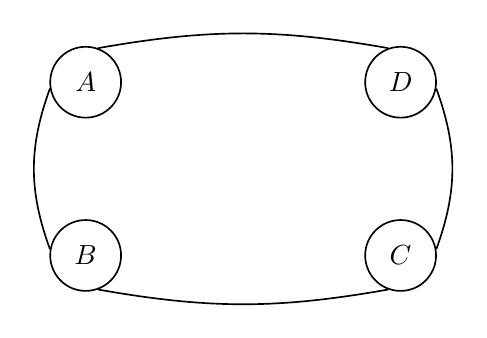
\begin{tikzpicture}[line width=.6pt,font=\normalsize]
\tikzset{repnode/.style={circle,draw,fill=white,minimum size=9mm,inner sep=0pt}}
\node[repnode] (A) at (0,2.2) {$A$};
\node[repnode] (D) at (4,2.2) {$D$};
\node[repnode] (B) at (0,0) {$B$};
\node[repnode] (C) at (4,0) {$C$};
\draw (A.70) to[bend left=10] (D.110);
\draw (D.350) to[bend left=20] (C.10);
\draw (C.250) to[bend left=10] (B.290);
\draw (B.170) to[bend left=20] (A.190);
\end{tikzpicture}